\begin{methods}
\section{Results}\label{sec:results}

\paragraph{LoRA adaptation dramatically improves expression prediction.}
Table~\ref{tab:results} summarizes expression prediction performance across all variants. With frozen \botanic embeddings, the best head variant (C, cross-attention + FiLM) achieves PCC\,=\,0.818 on log-scale expression but only PCC\,=\,0.401 on TPM-scale. LoRA adaptation of the foundation model transforms performance: the same simple concatenation head (Variant A) improves from PCC\,=\,0.744 to 0.910 (log) and from 0.124 to 0.816 (TPM). This demonstrates that task-specific fine-tuning is essential---frozen embeddings capture general sequence properties but miss expression-relevant features that LoRA adaptation recovers.

\paragraph{Simpler heads outperform complex architectures with strong embeddings.}
With LoRA-adapted embeddings, the simplest multi-modal head (Variant A, 1.0M params) outperforms the 10$\times$ larger cross-attention + FiLM model (Variant C, 10.6M params): PCC\,=\,0.910 vs.\ 0.904. This reverses the ranking observed with frozen embeddings, where architectural complexity compensated for weaker representations (C: 0.818 vs.\ A: 0.744). The result suggests that strong foundation model embeddings reduce the need for complex downstream architectures.

\paragraph{Sequence embeddings complement epigenomic features.}
Variant E (epigenomic features only, 0.65M params) achieves PCC\,=\,0.847, establishing that histone marks alone are predictive but insufficient. Adding \botanic embeddings (Variant A) improves PCC by +0.063 (log) and +0.162 (TPM), confirming that sequence context captured by the foundation model provides complementary information to chromatin state.

\paragraph{Comparison with DeepWheat.}
DeepWheat \citep{DeepWheat2024} trains separate per-tissue CNNs (24--54M params each, 245M total) on sequence and chromatin windows around each gene. To ensure a fair comparison, we loaded the pretrained DeepWheat models from their Zenodo repository and evaluated them on the same deterministic 80/10/10 test split used by \mytool (seed\,=\,42; Table~\ref{tab:deepwheat}). DeepWheat performs well on leaf (PCC\,=\,0.864) and spike (PCC\,=\,0.820), consistent with its published results, but generalizes poorly to developmental tissues: vl\,=\,0.111, e7\,=\,0.303, e9\,=\,0.287, with negative $R^2$ values indicating predictions worse than the tissue mean. The mean PCC across all six tissues is 0.461. By contrast, \mytool achieves PCC\,=\,0.910 uniformly across all tissues with a single 1.0M-parameter head---a 97\% mean improvement with 245$\times$ fewer parameters. DeepWheat's per-tissue architecture cannot share learned representations across tissues, which likely explains its failure on developmental tissues where training signal is sparser (50\% of genes are silent in e7/e9 vs.\ 41\% in leaf).

\begin{table}[!t]
\processtable{Per-tissue DeepWheat evaluation on \mytool test split.\label{tab:deepwheat}}{
\begin{tabular}{@{}lccr@{}}
\toprule
Tissue & PCC & $R^2$ & Params \\
\midrule
Leaf       & 0.864 &  0.740 & 37.8M \\
Spike      & 0.820 &  0.350 & 40.0M \\
e5         & 0.383 &  0.029 & 24.2M \\
e7         & 0.303 & $-$0.099 & 36.9M \\
e9         & 0.287 & $-$0.245 & 51.7M \\
vl         & 0.111 & $-$0.507 & 54.3M \\
\midrule
Mean       & 0.461 &  0.043 & 244.9M \\
\botrule
\end{tabular}}{All models evaluated on the same held-out test set (seed\,=\,42, 10\% of 117,319 genes). Negative $R^2$ indicates predictions worse than predicting the tissue mean. The spike model required architecture reconstruction from saved weight shapes due to a hyperparameter metadata error in the released files.}
\end{table}

\paragraph{Embedding structure reflects expression biology.}
PCA of LoRA-adapted embeddings reveals that the first principal component correlates strongly with mean expression level ($r$\,=\,$-$0.651), compared to $r$\,=\,$-$0.071 for frozen embeddings (Figure~\ref{fig:embeddings}). UMAP projections further show that LoRA embeddings organize genes into expression-coherent clusters, with clear separation between silent and highly expressed genes. This confirms that LoRA adaptation restructures the embedding space to encode expression-relevant information.

\paragraph{Epigenomic mark contributions.}
Analysis of histone mark--expression correlations reveals that H3K27ac and H3K9ac are the strongest positive predictors of expression ($r$\,=\,0.469), consistent with their known roles as active enhancer and promoter marks. H3K36me3 shows an anti-correlation ($r$\,=\,$-$0.285), likely reflecting its association with gene body methylation patterns in wheat. H3K27me3, a canonical repressive mark, shows the expected negative association ($r$\,=\,$-$0.228).

\begin{table}[!t]
\processtable{Expression prediction performance across head variants and embedding types.\label{tab:results}}{
\begin{tabular}{@{}llrcccc@{}}
\toprule
& & & \multicolumn{2}{c}{Log-scale} & \multicolumn{2}{c}{TPM-scale} \\
\cmidrule(lr){4-5} \cmidrule(lr){6-7}
Embed. & Head & Params & PCC & $R^2$ & PCC & $R^2$ \\
\midrule
\multirow{4}{*}{Frozen}
& A (concat) & 1.0M & 0.744 & 0.544 & 0.124 & 0.003 \\
& B (cross-attn) & 10.0M & 0.681 & 0.270 & 0.117 & 0.013 \\
& C (FiLM) & 10.6M & 0.818 & 0.664 & 0.401 & 0.142 \\
& D (contr.) & 10.6M & 0.803 & 0.621 & 0.185 & 0.030 \\
\midrule
\multirow{3}{*}{LoRA}
& E (epi-only) & 0.65M & 0.847 & 0.716 & 0.654 & 0.406 \\
& C (FiLM) & 10.6M & 0.904 & 0.817 & 0.810 & 0.647 \\
& \textbf{A (concat)} & \textbf{1.0M} & \textbf{0.910} & \textbf{0.826} & \textbf{0.816} & \textbf{0.655} \\
\midrule
\multicolumn{2}{l}{DeepWheat (mean$^\dagger$)} & 245M & 0.461 & 0.043 & --- & --- \\
\botrule
\end{tabular}}{PCC: Pearson correlation coefficient. $R^2$: coefficient of determination. $^\dagger$Mean of six per-tissue CNNs on the same test split; see Table~\ref{tab:deepwheat} for per-tissue breakdown.}
\end{table}

\begin{figure}[!tpb]
\centerline{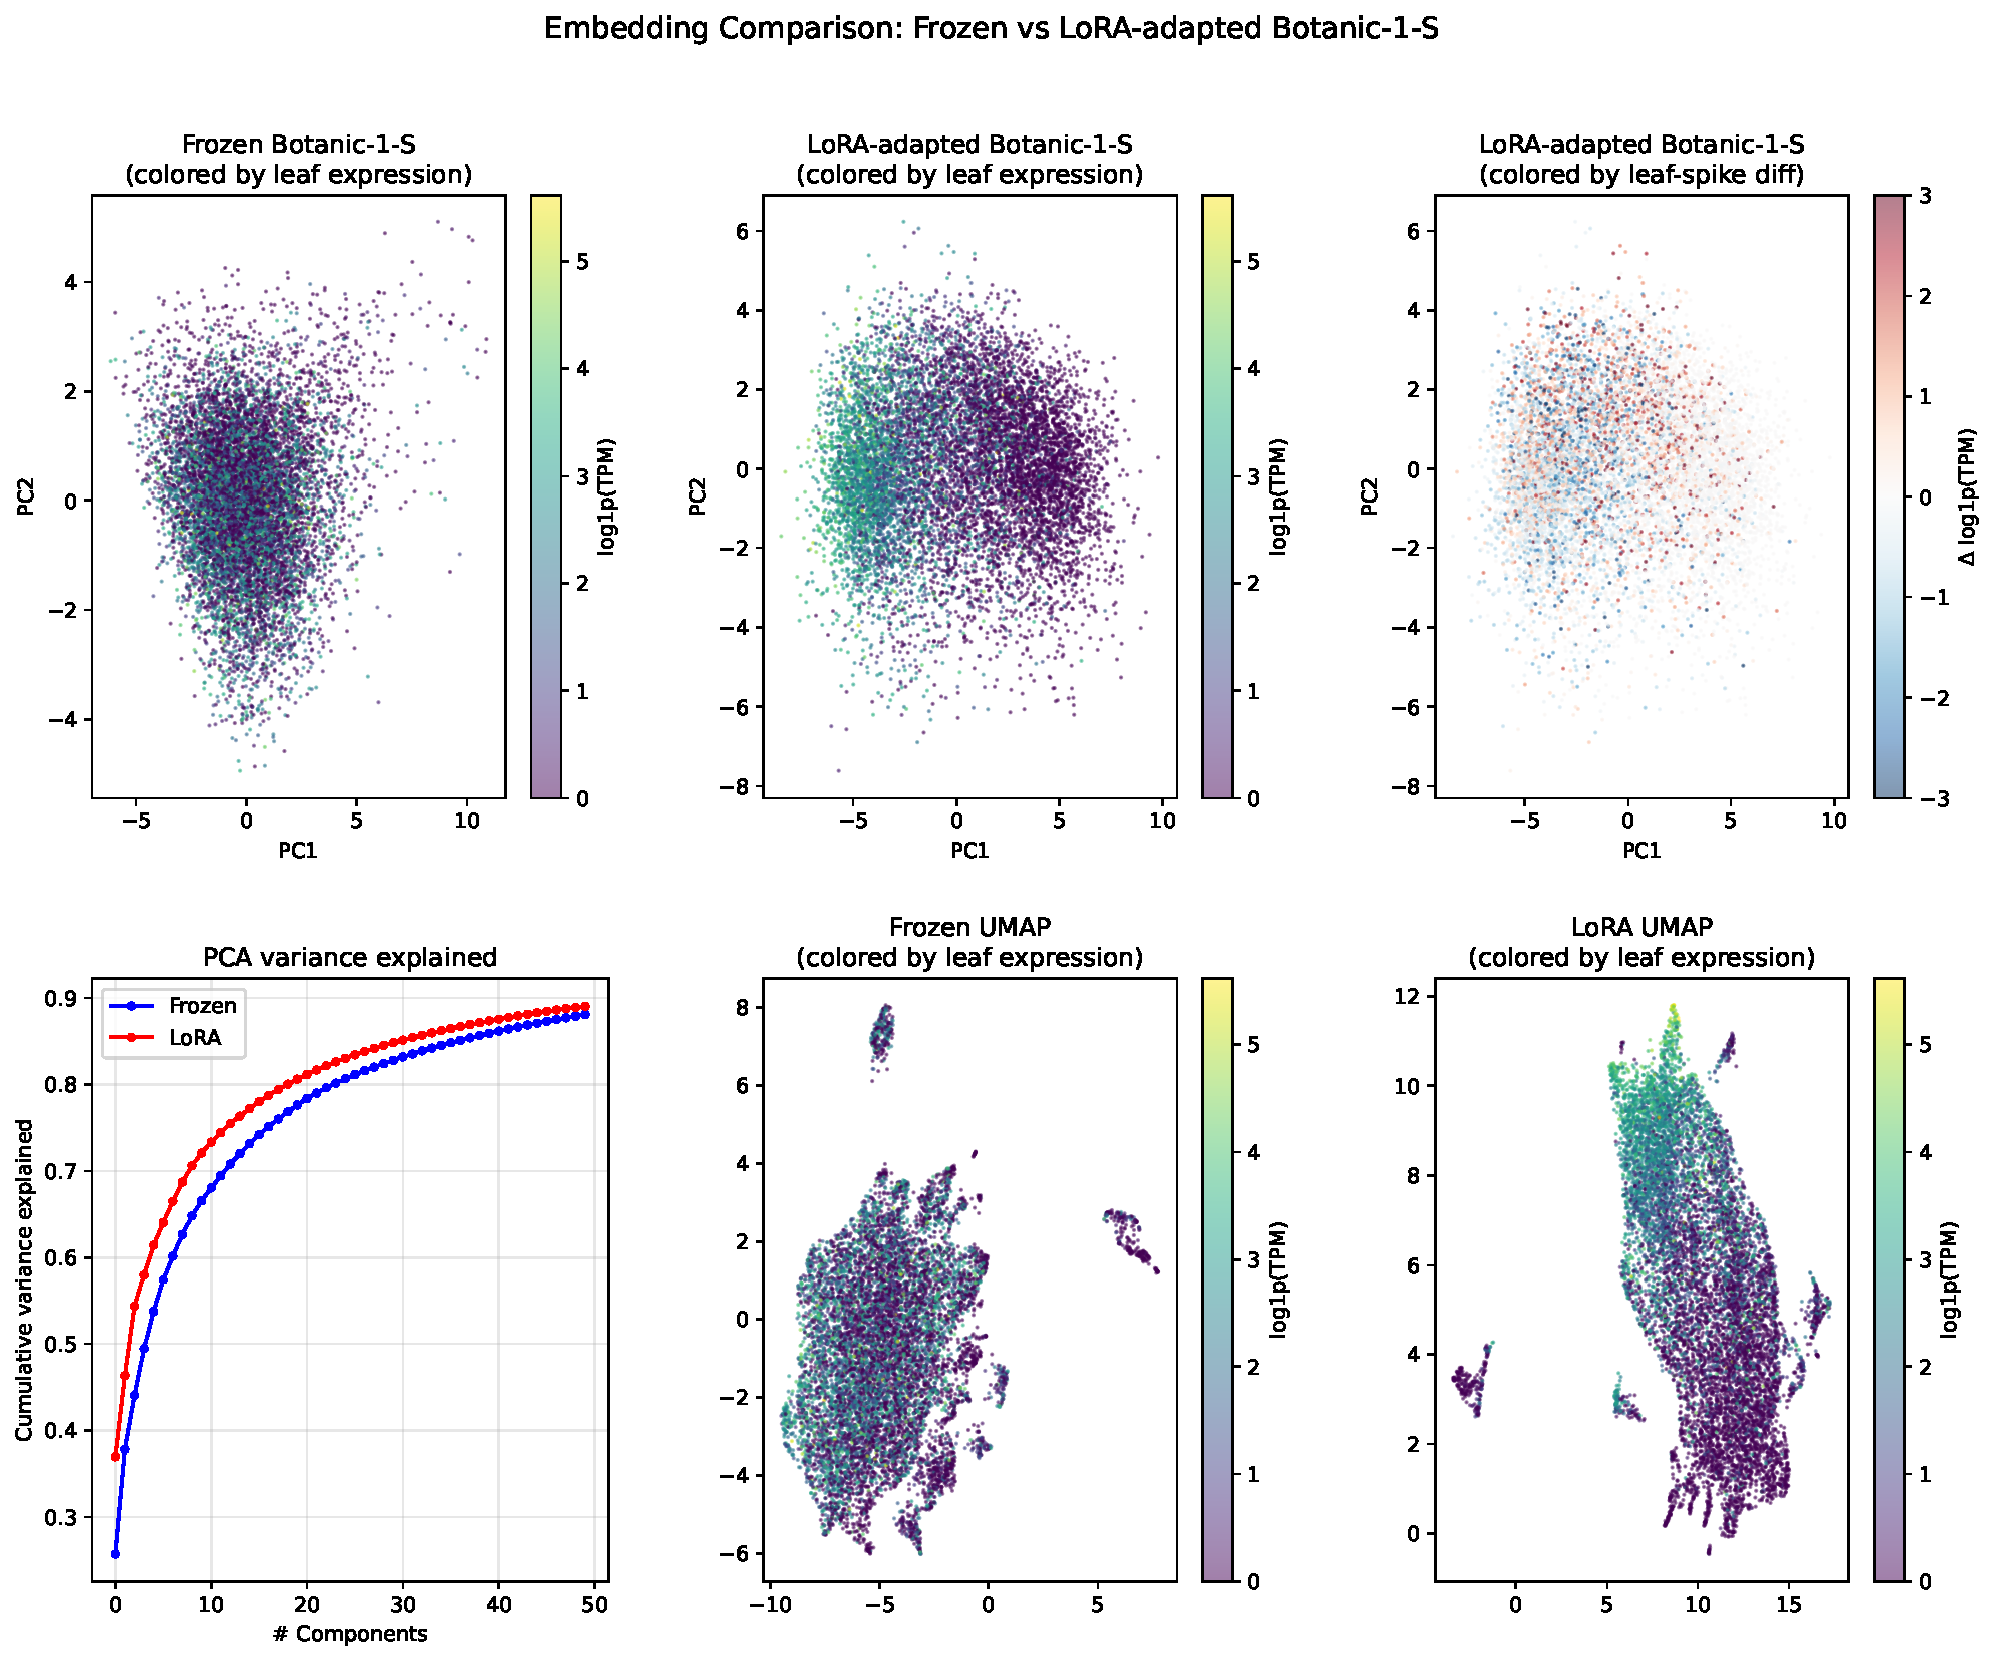
\includegraphics[width=\columnwidth]{figures/analysis1_embedding_comparison.pdf}}
\caption{PCA and UMAP of frozen vs.\ LoRA-adapted \botanic embeddings (5000 genes). Points are coloured by mean expression level. LoRA adaptation organizes the embedding space to reflect expression biology (PC1 $r$\,=\,$-$0.651 vs.\ $-$0.071 for frozen).}\label{fig:embeddings}
\end{figure}

\end{methods}
